\chapter{Estimating the luminosity}\label{chap:luminosity}

%\epigraph{As for their appearance, the four of them looked alike; each was like a wheel intersecting a wheel. Their entire bodies, including their backs, their hands and their wings, were completely full of eyes, as were their four wheels.}{Ezekiel,10:10-12}
\section{Concept of luminosity}
In particle physics experiments, the energy available for producing new particles is a crucial parameter. The most efficient configuration is given by colliding two beams of equal energy head to head. Thus, the energy available in the system corresponds to the centre of mass energy of the two colliding beams.

Another critical aspect is the number of interactions referred to as ``events", especially when studying rare processes with a small production cross-section $\sigma_p$. The ability of a particle accelerator to produce the required number of interactions is quantified by the concept of luminosity, defined as the proportionality factor between the number of events per second $\tfrac{dR}{dt}$ and the cross-section. The relation between luminosity $\mathcal{L}$, cross-section $\sigma_p$ and rate $\tfrac{dR}{dt}$ is:
\begin{equation}
    \frac{dR}{dt} = \mathcal{L}{\sigma_p}\label{lumi_def}
\end{equation}
The unit of luminosity is therefore $\SI{}{\per\centi\meter\squared\per\second}$.
 
Let us define the average number of events in a visible process $\mu_{\text{vis}}$ as:

\begin{equation}
\mu_{\text{vis}} = \frac{\Rho_{\text{vis}}}{f} = \frac{\mathcal{L} \sigma_{\text{vis}}}{f}\label{mu_def}
\end{equation}

where:
\begin{itemize}
\item  $\Rho_{\text{vis}}=\tfrac{dR}{dt}$ is the interaction rate of a visible process,
\item  $f$ is the frequency of collisions,
\item  $\mathcal{L}$ is the instantaneous luminosity,
\item  $\sigma_{\text{vis}}$ is the cross section of the chosen visible process.
%, and
%\item  $\mu_{\text{vis}}$ represents the average number of visible processes. %proton-proton (pp) interactions per crossing.
\end{itemize}
The relation \eqref{mu_def} can be used to measure luminosity indirectly by determining $\mu_{\text{vis}}$ from processes of known cross section $\sigma_\text{vis}$.
%, such as those producing at least two reconstructed VELO tracks. 
Once $\mu_{\text{vis}}$ is measured, the luminosity is derived as follows:

\begin{equation}\label{rel_lumi}
\mathcal{L} = \frac{\mu_{\text{vis}} \cdot f}{\sigma_{\text{vis}}}
\end{equation}

This approach is referred to as ``relative luminosity determination" because it relies on the known visible cross section $\sigma_{\text{vis}}$ to ``calibrate" the luminosity, using it as a normalisation factor. During periods of data taking at LHCb, different ``luminosity counters" record the amounts of visible interactions, allowing to calculate $\mu_{\text{vis}}$. This data is then used to estimate the instantaneous luminosity with the various counters that will be presented in Section \ref{sec:luminometers}, enabling accurate cross-section measurements and experiment calibration.


% Integrated Luminosity Definition
The maximum luminosity, and therefore the maximal instantaneous number of interactions per second, is a significant factor in particle collider experiments, especially in LHCb as it will explained in Section~\ref{sec:lumi_levelling}. However, the final figure of merit for the number of recorded collisions is the integrated luminosity, denoted by $\mathcal{L}_{\text{int}}$. Over a given time period $T$, it is defined as:

\begin{equation}
\mathcal{L}_{\text{int}} = \int_0^T \mathcal{L}(t) dt .
\end{equation}
Integrated luminosity is useful because it directly relates with the total number of events of interest:

\begin{equation}
\mathcal{L}_{\text{int}} \times \sigma_p = \text{number of events of interest}.
\end{equation}

The unit of integrated luminosity is therefore $\SI{}{\per\centi\meter\squared}$, but more often the barn unit is used, which is defined as $\SI{1}{\barn}=\SI{1e-24}{\per\centi\meter\squared}$. The integrated luminosity indicates the quantity of data available for analysis.

% Luminosity Decay Model
A factor influencing integrated luminosity is the decay of instantaneous luminosity over time, caused by various factors like beam intensity reduction, transverse emittance growth, and bunch length increase. A common model to represent this decay assumes an exponential form:
\begin{equation}
\mathcal{L}(t) = \mathcal{L}_0 \exp\left( -\frac{t}{\tau} \right)
\end{equation}
where $\mathcal{L}_0$ is the initial luminosity, $t$ is the elapsed time, and $\tau$ is the lifetime associated with the luminosity decay. 

In the following paragraphs, the formula that is widely used for computing the luminosity at a collider experiment will be derived.
Subsequently, I will describe the luminosity at LHCb and explain how at this experiment we can avoid luminosity decay by introducing the luminosity levelling procedure. The process of ``calibrating" the counters, i.e. calculating the visible cross section $\sigma_{\text{vis}}$, is carried out in a procedure called van der Meer Scan, that will be presented from a theoretical point of view in Section \ref{sec:calibration_vdm}. In Section~\ref{lumi_measure} I will finally introduce the counters used in this thesis and explain how the calibration has been carried out, as well as showing the rationale behind combining them to obtain an overall single luminosity measurement.

\paragraph{Luminosity in fixed target experiments}
In fixed target experiments, luminosity is influenced by the properties of both the incoming beam and the stationary target. The incoming beam is characterised by its flux $\Phi$, which is the number of particles per second. Let us consider an homogeneous target thin enough to let only a small fraction of beam particles actually
interact, so we can assume that $\Phi$ is constant. We define the number of scattering centres $n_T$ as the number of particles of the target with which the beam interacts. This quantity is given by multiplying the atomic density $\rho_T$ of the target with its length $l$.  
The rate of the process is easily found by using the cross section $\sigma_p$ of the process:

\begin{equation}
\frac{dR}{dt} =\Phi \cdot n_T \cdot \sigma_p = \Phi \cdot \rho_T \cdot l \cdot \sigma_p\label{rate_fixed_target}
\end{equation}

The luminosity in this setup follows directly from \eqref{rate_fixed_target} and the luminosity definition in \eqref{lumi_def}:

\begin{equation}
\mathcal{L}_{FT} = \frac{dR}{dt}\frac{1}{\sigma_p} = \Phi \cdot \rho_T \cdot l
\end{equation}

\paragraph{Luminosity in collider experiments}
In colliding beam experiments, both beams act as the target and the incoming beam simultaneously. The general expression for luminosity in this case involves the convolution of the 3D distribution functions of the protons in the beams, considering the overlap integral. A schematic picture is shown in Figure \ref{fig:lumi-def}\cite{Herr:941318}. Since the two beams are not stationary but moving through each other, the overlap integral depends on the longitudinal position of the bunches, and therefore on time, as they move towards and through each other. For our integration we use the distance of the two beams to the central collision point $s_0 = ct$ as the ”time” variable. 
The luminosity is proportional to the overlap integral of the two time dependent beam densities  $\rho_1$, $\rho_2$:

\begin{figure}
    \centering
    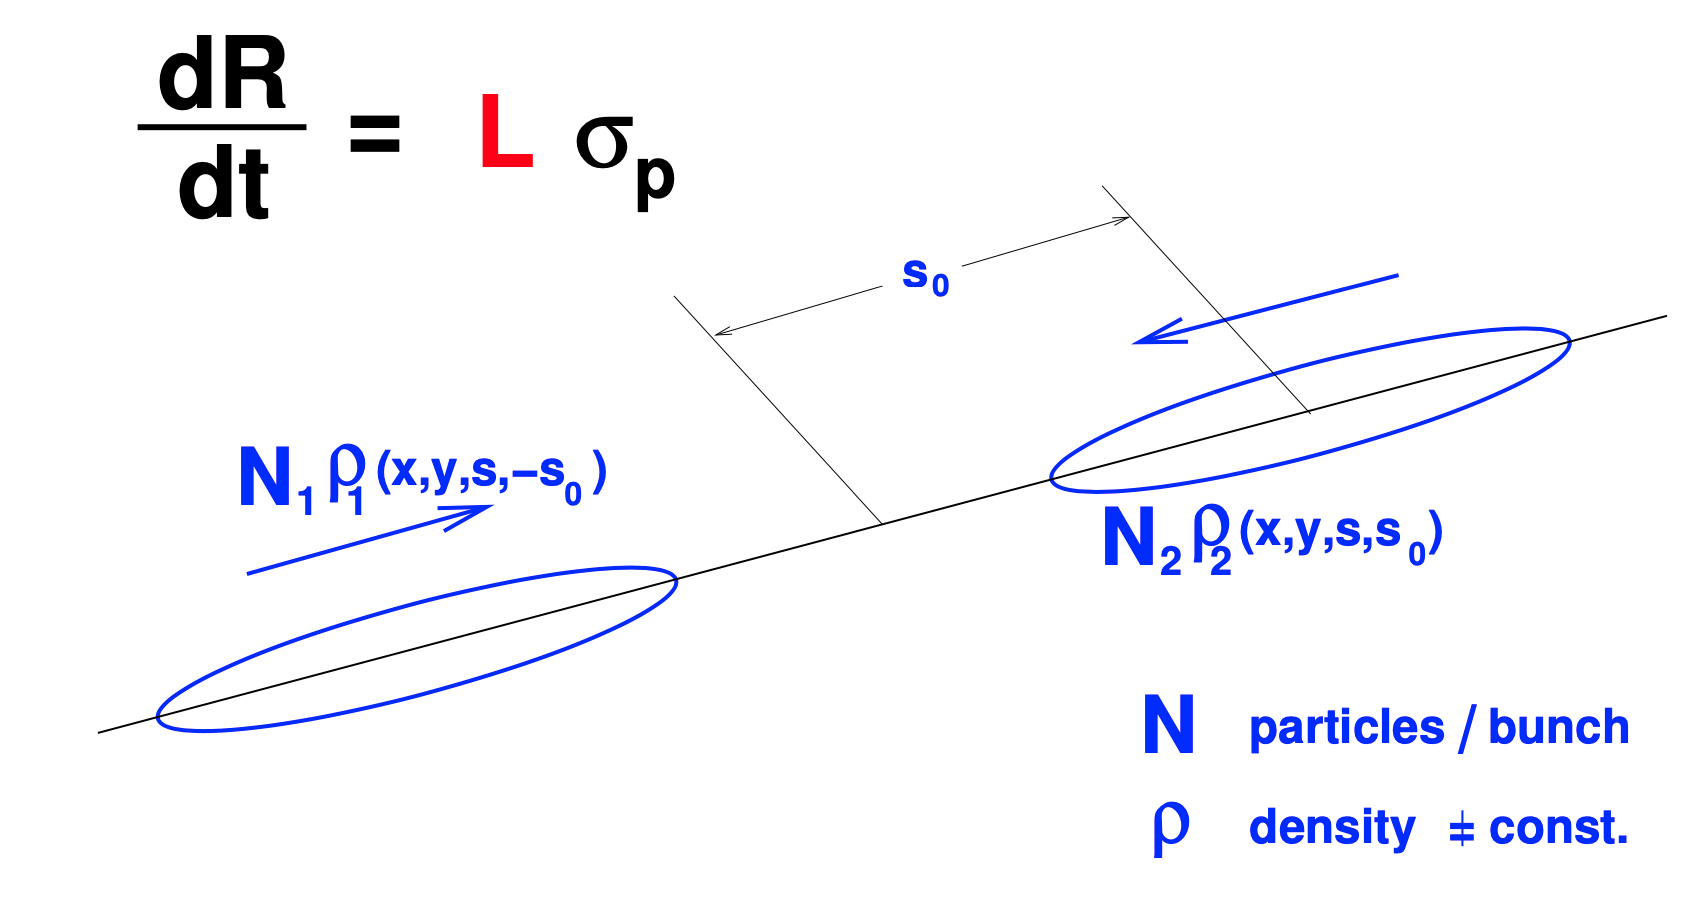
\includegraphics[width=0.6\textwidth]{figures/luminosity_def.png}
    \caption{Schematic view of a colliding beam interaction.}
    \label{fig:lumi-def}
\end{figure}

\begin{equation}
    \mathcal{L} \propto K\cdot\iiiint_{-\infty}^{+\infty}\rho_1(x,y,s,s_0)\rho_2(x,y,s,s_0)dxdydsds_0.\label{lumi_propto}
\end{equation}
Assuming the bunches collide at $s_0$, we have to take into account the kinematic factor\cite{Moller}:
\begin{equation}
    K = \sqrt{\bigl(\vec{v_1}-\vec{v_2}\bigr)^2-\bigl(\vec{v_1} \times \vec{v_2}\bigr)^2}/c.
\end{equation}
By further assuming head-on collisions ($\vec{v_1}=-\vec{v_2}$) in the relativistic limit ($K=2$) and that all densities are uncorrelated in all planes, we can write:
\begin{equation}
        \mathcal{L} = 2 N_1 N_2 f N_b\cdot\iiiint_{\infty}^{+\infty}\rho_{1x}(x)\rho_{1y}(y)\rho_{1s}(s-s_0)\rho_{2x}(x)\rho_{2y}(y)\rho_{2s}(s+s_0)dxdydsds_0.\label{beam_overlap}
\end{equation}
where:
\begin{itemize}
    \item $ N_1$  and $N_2$  are the number of particles per bunch for each beam;
    \item $f$ is the revolution frequency;
    \item $N_b$  is the number of bunches in each beam.
\end{itemize}

To evaluate this integral one should know the bunch densities. An analytical calculation is not always possible and a numerical integration may be required. However in many cases the beams have ``reasonable” profiles and we can obtain closed solutions. It is often assumed that the beam profiles follow Gaussian distributions. This assumption is justified because the luminosity is determined by the overlap of the core of the distributions, with the tails contributing minimally.
Given Gaussian profiles, we can write the distribution function for a Gaussian bunch in a general form:
\begin{equation}
\rho_{ik}(k) =\frac{1}{\sigma_{ik}\sqrt{2\pi}} \exp\left( -\frac{k^2}{2 \sigma_{ik}^2} \right) \text{ where } i=1,2, \quad k=x,y
\end{equation}
\begin{equation}
\rho_{s}(s\pm s_0) =\frac{1}{\sigma_s\sqrt{2\pi}} \exp\left( -\frac{(s\pm s_0)^2}{2 \sigma_s^2} \right)
\end{equation}
Let us assume equal beams, i.e.  $\sigma_{iz} = \sigma_{jz}$ for $i=j$, $k=x,y,s$ and that the number of particles per bunch $N_1$ and $N_2$, revolution frequency $f$, and number of bunches $N_b$ are known. 

Using this information, the luminosity integral can be derived by first considering the overlap integral of the Gaussian distributions as in equation \eqref{beam_overlap}:

\begin{equation}
\mathcal{L} = \frac{2\  N_1\ N_2\ f\ N_b}{(\sqrt{2\pi})^6\ \sigma_x^2\ \sigma_y^2\ \sigma_s^2}\iiiint e^{-\frac{x^2}{ \sigma_x^2}} e^{-\frac{y^2}{\sigma_y^2}} e^{-\frac{s^2}{\sigma_s^2}}e^{-\frac{s_0^2}{\sigma_s^2}}dxdydsds_0.
\end{equation}
Integrating over $s$ and $s_0$, we get a first intermediate result\footnote{integral of a gaussian pdf: $\int_{-\infty}^{+\infty}e^{-at^2}dt = \sqrt{\tfrac{\pi}{a}}$}:
\begin{equation}
    \mathcal{L} = \frac{2\  N_1\ N_2\ f\ N_b}{8(\sqrt{\pi})^4\ \sigma_x^2\ \sigma_y^2}\iint \exp\left(-\frac{x^2}{\sigma_x^2}\right) \exp\left(-\frac{y^2}{\sigma_y^2}\right) dxdy .\label{spec_lumi_gaus}
\end{equation}
Finally, after integration over $x$ and $y$, we get the well-known formula of luminosity for colliding Gaussian beams with head-on collisions:

\begin{equation}
\mathcal{L} = \frac{N_1  N_2  f N_b}{4 \pi  \sigma_x \sigma_y}.
\end{equation}

%If we generalize to the case where the x and y beam profiles are unequal but still assume approximately equal bunch lengths (\( \sigma_{1s} \approx \sigma_{2s} \)), we get a modified formula for luminosity:

%\begin{equation}
%\mathcal{L} = \frac{N_1  N_2  f  N_b}{2 \pi \sqrt{(\sigma_{1x}^2 + \sigma_{2x}^2)(\sigma_{1y}^2 + \sigma_{2y}^2)}}.
%\end{equation}


\section{Luminosity at LHCb}
%A critical parameter for LHCb performance is the average number of interaction $\mu$, defined in Eq. \eqref{mu_def}.
The LHCb experiment focuses on investigating heavy flavour physics, probing for new physics phenomena in $\mathcal{CP}$ violation and rare decays of $b$-quark and $c$-quark hadrons. This exploration relies heavily on the precise reconstruction of primary and secondary vertices and the complete topology of the decay chains. The reconstruction of vertices can suffer from high pile-up $\mu$, i.e. the number of $pp$ collisions for each bunch crossing, that increases combinatorial background and complicates track reconstruction.

For this reason, LHCb was initially designed to operate at a luminosity of \SI{2e32}{\per\centi\meter\squared\per\second} corresponding to an average pileup $\mu\sim0.4$. This luminosity is lower that the one that LHC reaches and supply to ATLAS and CMS. By design, the beams in LHC are defocused before reaching the LHCb interaction point, in order to decrease the value of luminosity and let our experiment operates at its optimal conditions. A fundamental but extremely challenging turn point in the operational strategy of LHCb came when the LHC changed approach in June 2010 from commissioning many bunches with low intensity to rather commissioning nominal (and above) intensity per bunch. The average event pileup in LHCb quickly reached $\mu \approx 2.5$. Even in this exceptionally high pileup environment, it was shown that the majority of the LHCb systems performed extremely well \cite{det_perf}.
%In late 2009, LHCb recorded its first proton-proton (pp) collisions at an injection energy of $\sqrt{s}=\SI{0.9}{\tera\eV}$. 
%These data were used to finalise the commissioning of the sub-detector systems, calibration, and the alignment of tracking, calorimeter, and particle identification (PID) systems. During this period, the VELO was left in the open position to accommodate the larger aperture required at lower beam energies.

%The operating conditions changed rapidly in 2010 due to the LHC ramp-up in luminosity.  Luminosity started around $\sim \SI{1e28}{\per\centi\meter\squared\per\second}$ with almost no pile-up but eventually reached $\sim \SI{1e32}{\per\centi\meter\squared\per\second}$ with .
%While the highest luminosity in 2010 was already 75\% of the LHCb design luminosity, the pile-up was much larger due to the low number of bunches in the machine. Despite this, the trigger and reconstruction systems demonstrated efficient performance under these conditions.

%\begin{figure}
%    \centering
%    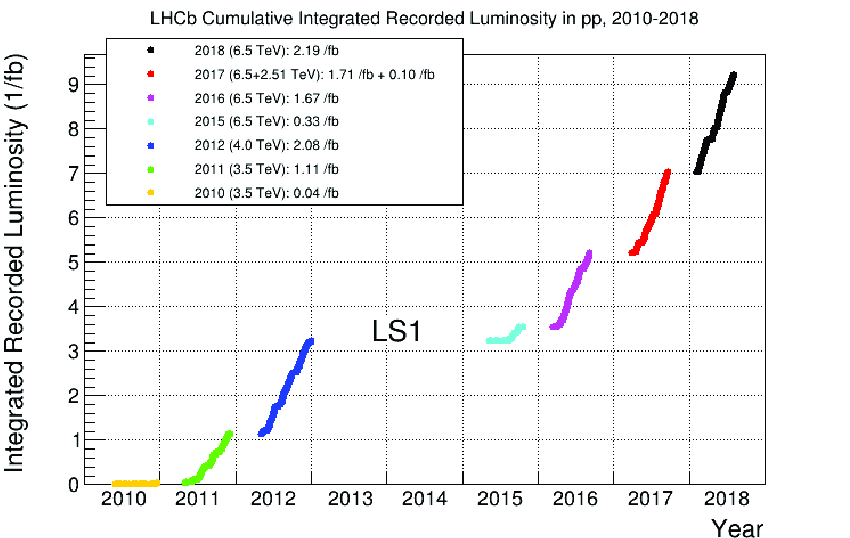
\includegraphics[width=\textwidth]{figures/lumiRun2.png}
%    \caption{Integrated luminosity during Run1 and Run2, interspersed by the LS1.}
%    \label{fig:lumiRun1Run2}
%\end{figure}

In 2011, the number of bunches in the machine increased to about 1300, allowing for a reduction in pile-up while LHCb operated at a luminosity of $\SI{3.5e32}{\per\centi\meter\squared\per\second}$. This was 1.75 times the design luminosity of $\sim \SI{2e32}{\per\centi\meter\squared\per\second}$. %The instantaneous luminosity directly delivered by the LHC was too high with respect to the target luminosity the LHCb experiment has been designed for, since of the too high event rate and irradiation dose to which the detectors would be subjected. Since of the higher detector hits multiplicity, track and vertex reconstructions would suffer of high event pile-up, that increases combinatorial background and complicates track reconstruction.

Since LHCb was already operating a defocus of the bunches, the collaboration decided to regulate the focusing in order to maintain a constant value for luminosity. In 2011, the experiment introduced a luminosity levelling procedure at the LHCb interaction point to keep the instantaneous luminosity stable within about 5\% during a fill. This was achieved by adjusting the transverse overlap of the beams, as it will be better explained in the next subsection.
%For one particularly long fill, a maximum overlap with head-on beams was reached only after 15 hours. This levelling minimised the effects of luminosity decay and allowed LHCb to maintain a consistent trigger configuration, reducing systematic uncertainties due to changing detector occupancy.

In 2012, the LHC beam energy was increased to $\SI{4}{\tera\eV}$, and LHCb took data at a luminosity of $\sim \SI{4e32}{\per\centi\meter\squared\per\second}$, twice the LHCb design luminosity. An effort was made in 2012 to use more efficiently the processing power available in the Event-Filter-Farm (EFF), deferring a fraction of the HLT processing to the inter-fill time ($\sim$ several hours) between the LHC collision periods. The experiment managed therefore to over-perform at a larger-than-design luminosity throughout Run~2.  
%in order to cope with the increase in luminosity, allowing LHCb to increase the data sample available for physics analysis. 


For Run~3, LHCb plans to reach an instantaneous luminosity of $\SI{2e33}{\per\centi\meter\squared\per\second}$, corresponding to a pile-up $\mu=5.5$.
%An overview of the luminosity integrated until the end of Run 2 is depicted in Figure \ref{fig:lumiRun1Run2}.
This goal is now affordable thanks to the renewed TDAQ system presented in Section \ref{sec:rta} and a complete renovation in the tracking system as explained in Section \ref{sec:detector}. 

Furthermore, the high-luminosity LHC project will bring LHCb to further increase the instantaneous luminosity reaching in Run~5 the peak value of $\mathcal{L}=\SI{2e34}{\per\centi\meter\squared\per\second}$ corresponding to an average pile-up $\mu=38$.

\subsection{Luminosity levelling}\label{sec:lumi_levelling}

Luminosity levelling is a crucial technique used by the LHCb experiment to stabilise the instantaneous luminosity and control pile-up at the experiment interaction point. It addresses the issue of excessively high event rates and irradiation doses caused by the high luminosity delivered by the LHC, which can complicate track reconstruction. Furthermore, it allows LHCb to maintain a consistent trigger configuration, reducing systematic uncertainties due to changing detector occupancy.

\begin{figure}
    \centering
    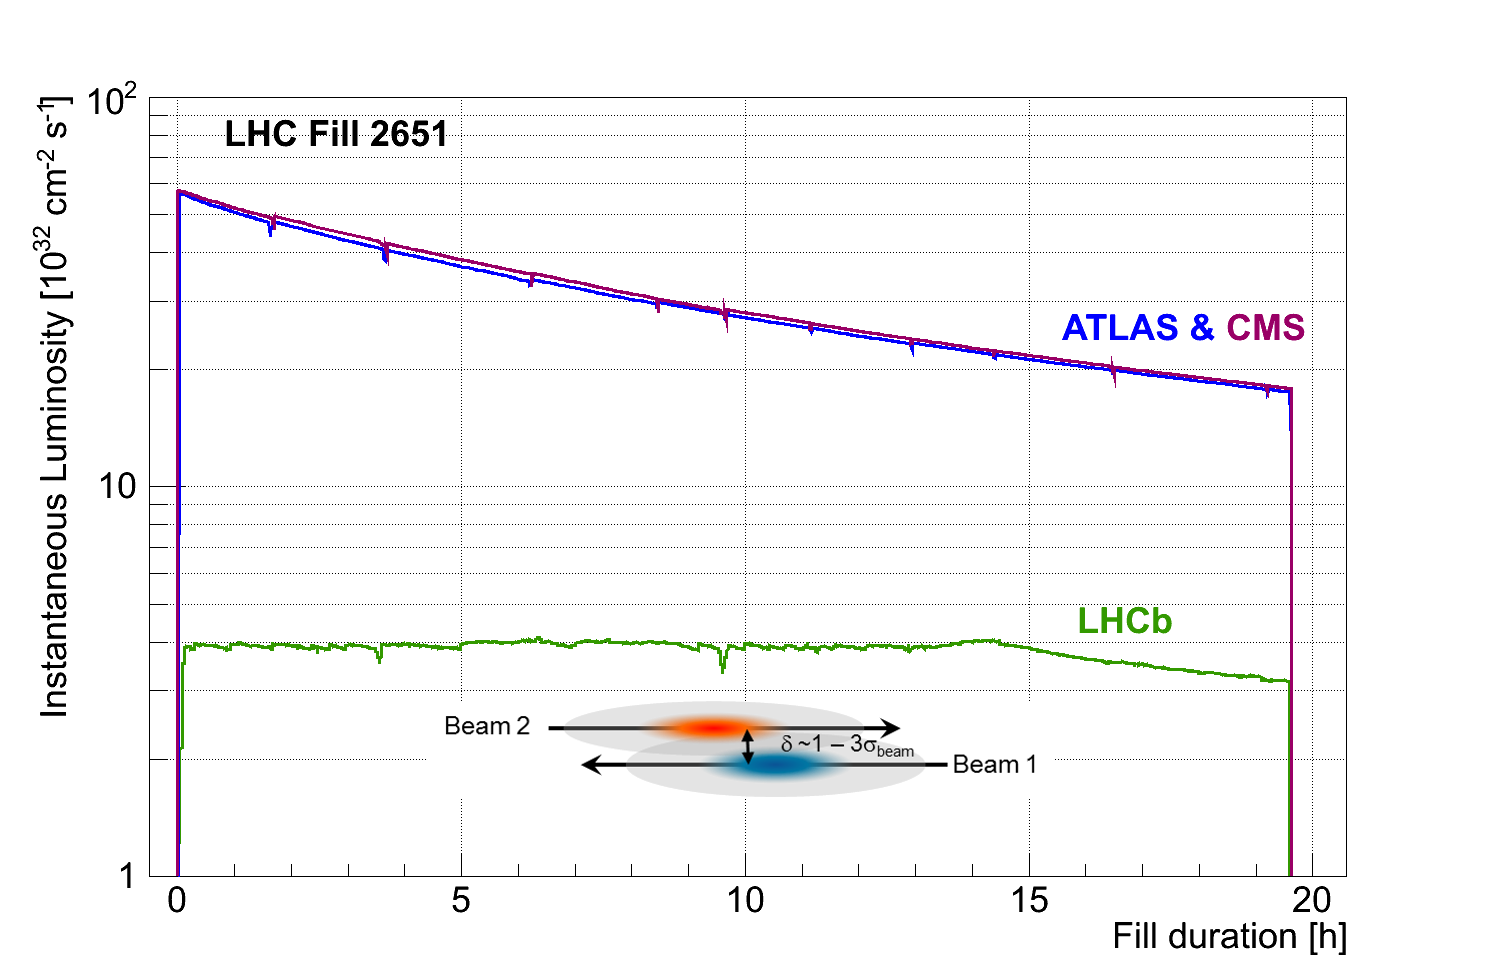
\includegraphics[width=0.8\textwidth]{figures/luminosity_leveling.png}
    \caption{Evolution of the instantaneous luminosity for ATLAS, CMS and LHCb during LHC fill 2651. After ramping to the desired value of $\SI{4e32}{\per\centi\meter\squared\per\second}$ for LHCb, the luminosity is kept stable in a range of 5\% for about 15 hours by adjusting the transversal beam overlap.
    The difference in luminosity towards the end of the fill between ATLAS, CMS and LHCb is due to the difference in the final focusing at the collision points, commonly referred to as the function $\beta^*$.}
    \label{fig:lumi-leveling}
\end{figure}

%The instantaneous luminosity in the LHCb experiment is kept constant at a lower value compared to other LHC experiments like CMS and ATLAS. 
Generally, the luminosity in an LHC fill follows an exponential decay trend due to beam intensity degradation effects. However, by using luminosity levelling, LHCb maintains the luminosity at a fixed peak value, allowing for consistent operational conditions for the DAQ and trigger systems.  This behaviour is well depicted in Figure \ref{fig:lumi-leveling}. For one particularly long fill, a maximum overlap with head-on beams was reached only after 15 hours. 


Luminosity levelling is achieved by adjusting the transverse overlap between the two colliding beams using corrector magnets located on each side of the experiment. The beam overlap is incrementally increased in small discrete steps as the beam intensity decreases, allowing for fine control of the luminosity. Precision in the online measurement of instantaneous luminosity is an important feedback to the LHC, needed in order to operate the luminosity levelling. It has been estimated that an accuracy of less than 5\% is sufficient for this purpose. 
 The adjustments are made through a luminosity control software, which provides feedback from the LHCb sub-detectors to the LHC Control Centre. A scheme of this software is reported in Figure \ref{fig:lumi-control}.
The LHCb luminosity control manager, part of the ECS, is a FSM driven by LHC operational modes. It monitors the instantaneous luminosity, compares it to the optimal target luminosity, and sends the levelling parameters to the LHC Lumi Levelling driver application. On the LHC side, this application uses a ``levelling algorithm" to determine the necessary adjustments in beam separation to maintain the target luminosity.

\begin{figure}
    \centering
    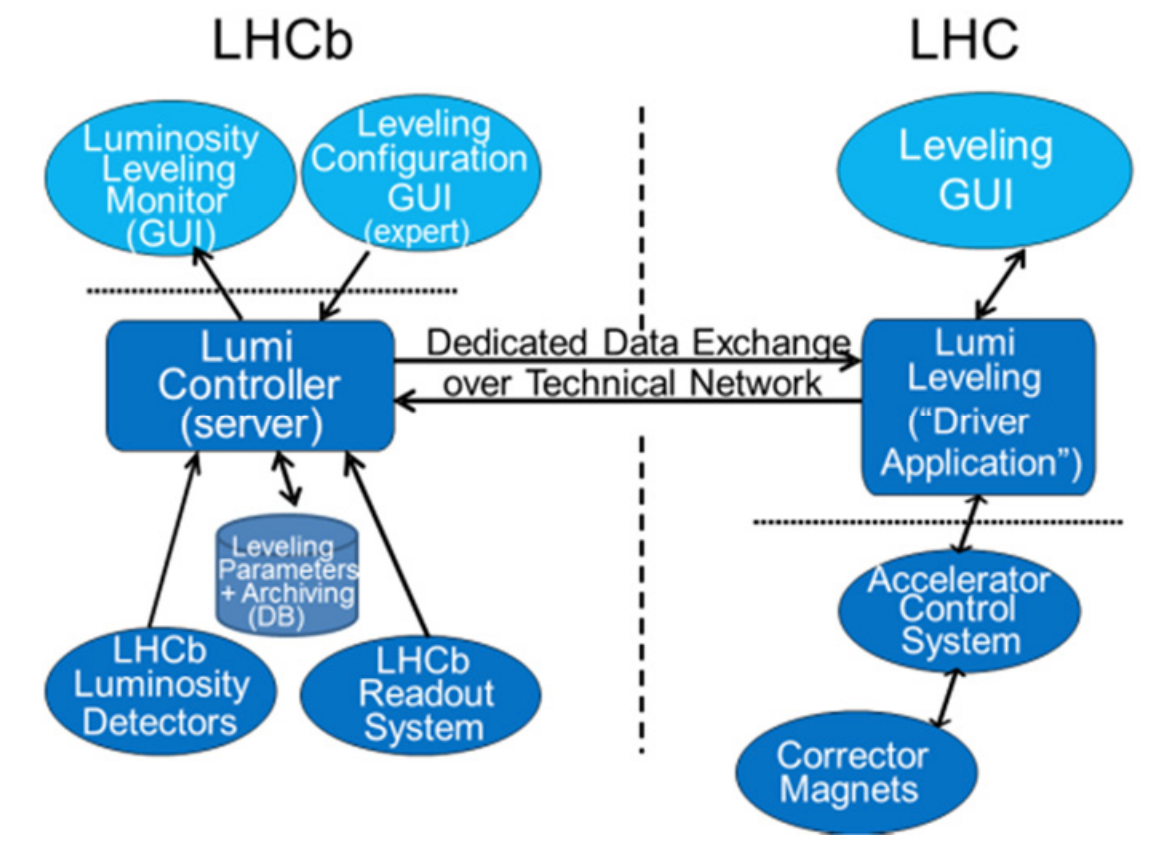
\includegraphics[width=0.5\textwidth]{figures/lumi_control.png}
    \caption{Diagram of the LHCb Luminosity control software}
    \label{fig:lumi-control}
\end{figure}

\subsection{Luminometers}\label{sec:luminometers}
The target luminosity for LHCb is a compromise between physics priorities, trigger selection efficiencies, detector performance limitations, DAQ system constraints, and offline data-processing capabilities. For Run~2, this value was set to $\SI{4e32}{\per\centi\meter\squared\per\second}$, while for Run~3, the target luminosity is estimated at $\SI{2e33}{\per\centi\meter\squared\per\second}$, corresponding to a pile-up per bunch-crossing of approximately $\mu = 5.5$.

During Run~1 and Run~2, online luminosity estimates had a precision of 10\% and were derived from two primary sources: 
\begin{enumerate}
    \item Transverse energy deposition: Observations of energy deposit over a fixed threshold in the calorimeter system;
    \item Muon station counts: Counts in the muon stations.
\end{enumerate}
Both of these quantities were available for the Level-zero L$0$ hardware-trigger.

As L$0$ was removed after Run~2, another subsystem was needed for the determination of the online luminosity in order to perform the lumi levelling. For this reason, the collaboration decided to implement a dedicated luminometer for the estimation of the luminosity in real-time, in order to perform the luminosity-levelling. In addition to PLUME, other luminosity counters working in real-time are implemented to serve as a cross-calibration and to be an eventual backup for PLUME.

During Run~2, the systematic uncertainty on the integrated luminosity was of 3.9\%, by far the principal source of systematics in most of the measurements of cross-sections (e.g.~\cite{j-psi}). The aim of the collaboration for Run~3 is to increase the precision in the integrated luminosity measurement, aiming at reaching an accuracy of 1\%\cite{Aaij:1951625}. 

For this reason, the collaboration decided to implement for Run~3 as many detector and systems as possible that will be used to determine an estimation of the integrated luminosity.
One approach is to count the number of reconstructed primary vertices per event $\nu$, which is directly proportional to the pile-up $\mu$, up to an acceptance-efficiency factor $\epsilon$. Another method is to measure count rates, such as the number of tracks per bunch crossing, hits on a detector, or reconstructed particles. These count rates exploits the method of ``relative luminosity determination" of equation~\eqref{rel_lumi}.

\subsubsection{PLUME}
A dedicated luminometer named PLUME (Probe for LUminosity MEasurement) was introduced for Run~3 to fill the fap left by the removal of L$0$ quantities  and provide feedback to LHC. PLUME consists of 24 hodoscopes (couples of detector modules read out in coincidence) surrounding the beam pipe, pointing at the nominal interaction point, and located approximately 1.7~meters upstream from the collision region. It covers a high-pseudorapidity range $(2.4 < \eta < 3.1)$.

Each hodoscope is composed of $10 \times 10 \times \SI{5}{\milli\meter\tothe{3}}$ quartz crystals, coupled with photomultipliers that detect Cherenkov light generated when high-speed particles traverse the quartz. Online luminosity measurement is performed by counting coincidences in at least one hodoscope, identifying tracks coming from the interaction region, and suppressing background activity.

A problem of linearity has been discovered in September 2022: due to a non-negligible rate of random coincidences the PLUME showed divergencies from the expected linear behaviour. Since July 7th 2022 PLUME luminosity corrected for non-linearity using HLT$1$ counters.
%, rendering de-facto PLUME an offline luminosity estimator.


\subsubsection{Other counters} 
In addition to the PLUME detector, LHCb introduced several other luminosity counters for online monitoring and offline luminosity measurement. This redundancy provides stability cross-checks and helps evaluate systematic uncertainties for the estimation of the integrated luminosity.
Secondly, some of these counters provide a backup in case of PLUME malfunctions.
\begin{itemize}
   %\item VELO superpixel ASICS counters;
   \item Number of muon hits in the muon stations (luMUONmeter)~\cite{Albicocco:2812716};
   \item VELO tracks and reconstructed primary vertices;
   \item Number of reconstructed SciFi tracks;
   \item Energy deposition in the ECal and HCal;
    \item Hits in the RICH$1$ and RICH$2$ detectors;

\end{itemize}
 VELO clusters counters based on FPGA have been added in the last year, and are the object of this thesis, that I will discuss in Section~\ref{lumi_measure}.

\section{An absolute luminosity calibration: the van der Meer scan}
Most of the luminometers that LHCb implemented rely on the ``relative luminosity determination" defined in equation~\eqref{rel_lumi}. This method is based on counting some quantity $\mu_{vis}$ that is directly proportional to the luminosity. In order to obtain the luminosity value from a counter, the visible cross-section $\sigma_{\text{vis}}$ of the counter must be known or meausured.

This quantity $\sigma_{\text{vis}}$ can be measured with the help of the van der Meer (vdM) method, a technique widely used in HEP to calibrate luminosity counters. The vdM method involves separatingthe beams in the transverse plane by a distance $\Delta x$, $\Delta y$ and measuring the average number of interactions $\mu$ between two colliding bunches. 
We can rewrite equation \eqref{spec_lumi_gaus} for a the two dimensional case
\begin{equation}
    \mathcal{L} = N_1 N_2 f N_b\iint \rho_1(x,y) \rho_2(x,y) dxdy,\label{generic_lumi}
\end{equation}
where $\rho_{1,2}(x,y)$ are the densities of the two colliding bunches in the transverse plane.
We can then combine \eqref{generic_lumi} and \eqref{mu_def} in order to write the average number of interactions $\mu$ normalised by the number of colliding bunches $N_1$, $N_2$. Assuming that the position of the second beam $2$ is fixed, we can write:

\begin{equation}
\frac{\mu (\Delta x,\, \Delta y)}{N_1N_2} = \frac{\sigma}{f} \frac{\mathcal{L}}{N_1N_2} = \sigma N_b \iint \rho _1(x_2 + \Delta x,\, y_2 + \Delta y) \rho _2(x_2,y_2) dx_2\, dy_2, \label{vdm_1}
\end{equation}
where the subscript 2 of the coordinates $x_2$, $y_2$ refers to the stationary second beam.
%, $\mathcal{L}$ is the instantaneous luminosity and $\rho_{1,2}(x,y)$ the normalised transverse particle densities of the unseparated bunches.

Integrating both sides over $\Delta x$ and $\Delta y$ drastically simplifies \eqref{vdm_1} since
\begin{equation} \iiiint \rho _1(x_2 {+} \Delta x,\, y_2 {+} \Delta y) \rho _2(x_2,y_2) dx_2\, dy_2\, d\Delta x\, d\Delta y {=} 1, \label{vdm_2} \end{equation}
as can be easily proved by substituting $x_2+\Delta x\equiv x_1,\ y_2+\Delta y\equiv y_1$. In the new variables the integrals $\iint \rho _1(x_1,\, y_1)dx_1\,dy_1$ and $\iint \rho _2(x_2,\, y_2)dx_2\,dy_2$ decouple and reduce to unity by definition.

From \eqref{vdm_1} and \eqref{vdm_2} we obtain the vdM formula:
\begin{equation}
     \sigma = \frac{1}{N_b} \iint \frac{\mu (\Delta x,\, \Delta y)}{N_1N_2} d\Delta x\, d\Delta y= \iint \mu_{sp}(\Delta x,\, \Delta y)d\Delta x\, d \Delta y \label{sigma_vdm}
    \end{equation}

where we defined the specific number of interactions
\begin{equation}
\mu_{sp}=\frac{\mu}{N_1 N_2}\frac{1}{N_b}.\label{mu_sp}
\end{equation}

The derivation of \eqref{sigma_vdm} uses only $\mu _{sp}$ but not $\mu$ or $N_{1,2}$ separately. Therefore, it remains valid even if $\mu$ and the product $N_1N_2$ change arbitrarily but proportionally during the scan, e.g. due to a gradual decrease of beam currents with time. It is required, however, that $\rho_{1,2}$ remain constant.

Achieving precise parallel translations of particle beams in the transverse plane requires complex configurations of magnets. To translate a single beam in one direction, four magnets are needed, positioned at the corners of a trapezoid-shaped trajectory. Consequently, for steering two beams in both transverse directions, a total of 16 magnets are necessary at each interaction point. Given this complexity, ensuring consistent and synchronised movement of all magnets becomes challenging.

Due to these synchronisation difficulties, continuous scans are generally avoided in favour of a step-wise approach. At the LHC, for example, the specific interaction rate $\mu_{sp}(\Delta x,\Delta y)$ is measured at predefined discrete points. As beams are moved from one point to another, the process waits until the slowest magnet reaches its designated current value before starting the counting measurement.

In accelerator physics, it is common for particle beams to oscillate in the transverse plane due to beam optics elements (i.e. the quadrupoles) designed to keep particles on a stable trajectory. This phenomenon shapes the transverse bunch widths and determines the density profiles $\rho _{1,2}(x, y)$. However, the accelerator is designed to maintain separate stability and independence for oscillatory motions along the transverse components $x$ and $y$. Any coupling between coordinates risks introducing additional resonances in the oscillatory motions.

The density profiles $\rho _{1,2}(x, y)$ can therefore be factorised into $x$ and $y$ components:
\begin{equation}
\rho _{1,2}(x, y) = \rho _{1,2}^x(x) \cdot \rho _{1,2}^y(y).
\end{equation}
This allows the specific interaction rate $\mu_{sp}(\Delta x, \Delta y)$ to be similarly factorised:

\begin{equation}
\mu _{sp}(\Delta x, \Delta y) = \mu ^x_{sp}(\Delta x) \cdot \mu ^y_{sp}(\Delta y).
\end{equation}
Given this factorisation, the overlap integral becomes easier to calculate by reducing it to a product of one-dimensional integrals  along the lines $\Delta x = \Delta x_0$, $\Delta y = \Delta y_0$:
\begin{equation}
\sigma = \frac{\int \mu _{sp}(\Delta x, \Delta y_0)\, d\Delta x \times \int \mu _{sp}(\Delta x_0, \Delta y)\, d\Delta y}{\mu _{sp}(\Delta x_0, \Delta y_0)}.\label{definition_sigma_vdm}
\end{equation}
The integrals in numerator can be measured in two one-dimensional scans over $\Delta x$ at fixed $\Delta y_0$ and vice versa. The formula is valid for any point $(\Delta x_0, \Delta y_0$), but it might be advantageous to choose $(\Delta x_0, \Delta y_0$) not far from the point of maximum luminosity in order to collect a sufficient amount of interactions. This simplification is advantageous in a large-scale accelerator like the LHC because it allows for one-dimensional scans along $\Delta x$ and $\Delta y$, reducing beam time and minimising potential errors due to slow drifts in beam orbits. 
%The bias from not scanned coordinates is minimised at the maximum of $\mu$ where the derivative of e.g. $\mu_{sp}(\Delta x_0, \Delta_y)$ with respect to $\Delta x_0$ is zero.

While the XY factorisation provides a powerful framework for simplifying luminosity calibration, it is not always perfect. Imperfections in accelerator design or other factors can lead to coupling between $x$ and $y$ coordinates, which may affect the accuracy of the factorisation. These deviations are typically small but can introduce systematic errors in the calibration process.

To address this, the shape of the interaction region is studied to identify any signs of non-factorisability. If the projections of the luminous region profiles onto one coordinate remain invariant when scanning the other, the factorisation assumption holds. Otherwise, systematic corrections are required. Furthermore, any error in the beam displacements directly affects the cross-section. An accurate measurement of the $\Delta x, \Delta y$ scale is performed in a dedicated Length Scale Calibration (LSC), which always accompanies van der Meer scans. 

The best way to further improve accuracy is to perform two-dimensional scans, focusing on the central region where the majority of interactions occurs. This approach was pioneered at LHCb in 2017 and it can significantly reduce non-factorisation systematics and improve calibration accuracy\cite{Balagura_2021}.

Currently, at LHCb both in 1D and 2D scans are performed. An example of the steps performed in a 2D vdM scan is reported in Figure \ref{fig:vdm_steps_xy}, where is clearly visible the Turtle or Cherubim-like shape, hence the colloquial name ``turtle scan".

\begin{figure}
    \centering
    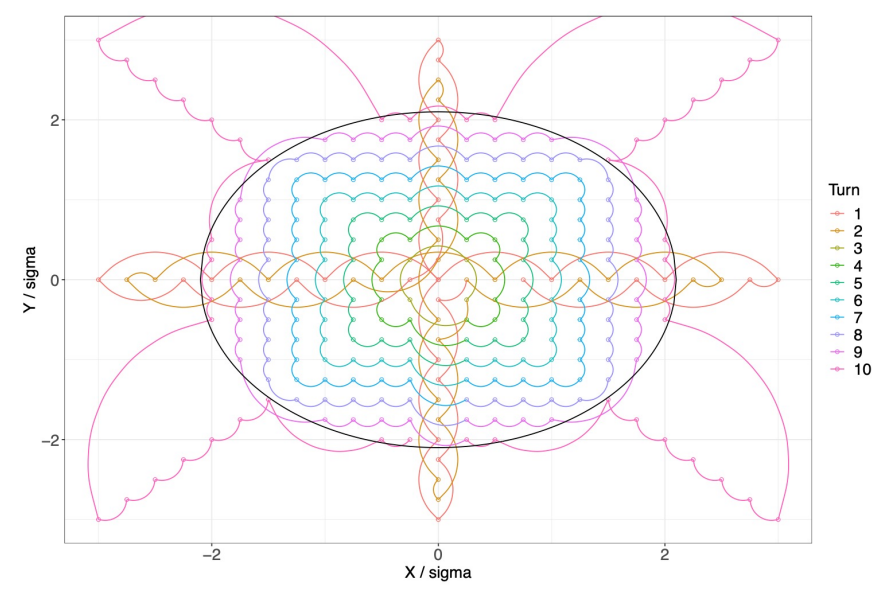
\includegraphics[width=0.7\textwidth]{figures/vdm_steps_xy.png}
    \caption{The displacements in x-y directions to perform a complete 2D van der Meer scan.}
    \label{fig:vdm_steps_xy}
\end{figure}



The step-wise scanning technique originated with van der Meer, who invented it over 50 years ago for the Intersecting Storage Rings (ISR) accelerator\cite{Carboni:156499}. Since then, it has been successfully applied with variations at other major accelerators\cite{Rubbia:1025746}, including the LHC. The method accuracy can range from 0.7\% to a few percent, establishing it as a reliable approach for luminosity calibration.

%Despite its success in hadron colliders, the van der Meer method can face challenges in electron-positron colliders due to strong beam–beam interactions. In these environments, luminosity is typically measured indirectly through Bhabha scattering events, where the quantum electrodynamics cross-section is well understood. In contrast, in hadron colliders, such as the LHC, it is harder to identify processes with accurately predicted cross-sections. Thus, in hadron accelerators, the best accuracy is typically achieved by directly measuring luminosity, following its definition.

\section{Online VELO Luminosity estimation}\label{lumi_measure}
The primitives described in Section~\ref{sec:velo_counters} are well suited to provide a relative luminosity measurement. In fact, we already stated various times in this chapter how a luminosity measurement can be obtained from simple counts, as defined equation~\eqref{rel_lumi}. The approach of performing a luminosity measurement from a pixel detector is not a novelty, but this method is rarely used. The only example found in literature regards an offline measurement by the CMS Collaboration~\cite{CMS-PAS-LUM-13-001}. With the accuracy that they reached, the CMS collaboration showed the potential on using pixel detectors fur such aims. 

From the 208 different counters implemented in the VELO, we could obtain 208 different luminosity measurements. 
In order to proceed, we need to:
\begin{itemize}
    \item verify the linearity of the counters with respect to the pile-up $\mu$ registered by LHCb;
    \item calibrate them calculating the $\sigma_{vis}$, as explained in Section \ref{sec:calibration_vdm};
    \item decide a robust procedure to combine them and provide a single overall luminosity measurement as precise as possible.
\end{itemize}

%A common method to measure luminosity in particle accelerators is through relative-luminosity measurements, which rely on the precise, event rate $\frac{dR}{dt}$ for a reference process. The basic formula, considering inelastic proton-proton (pp) processes with a cross section $\sigma_{inel}$, derives the expectation value of the instantaneous luminosity with respect to the revolution frequency, i.e. combining \eqref{lumi_def} and \eqref{mu_def}:
%\begin{equation}
%    \langle\mathcal{L}_{bunch}\rangle = \dfrac{\bigl<\frac{dR_{inel}}%{dt}\bigr>}{\sigma_{inel}} = \langle\mu_{inel}\rangle\frac{f_{rev}}%{\sigma_{inel}}
%\end{equation}
%
%The luminosity measurement can then be expressed as:
%\begin{equation}
%    \langle\mathcal{L}_{bunch}\rangle =  %\langle\mu_{vis}\rangle\frac{f_{rev}}{\sigma_{vis}}\label{lumi_per_bunch}
%\end{equation}
%
%where $\langle\mu_{vis}\rangle$ is the visible pile-up, which can be %calculated from the count rates or primary vertex measurements. The visible %cross-section $\sigma_{vis}$  accounts for the acceptance-efficiency factor, %with 
%$\sigma_{vis} = \epsilon \sigma_{inel}$
In principle, the average counts per event $\mu_{vis}$ provided by each counter are proportional to the luminosity (and therefore to the pile-up $\mu$). However, non-linearities can occur, particularly at high luminosity values, due to detector saturation or other factors. Therefore, intensive studies were performed on Monte Carlo simulations up to a pile-up $\mu = 28$, showing perfect linearity for our luminosity counters\cite{dan} with respect to the pile-up $\mu$. The linear behaviour is also confirmed on collision data in several fills. Particularly of interest is the case depicted in Figure \ref{fig:muscan}. In this particular conditions, the two beams are made collide one with the other at different overlap level. The LHC varies the pile-up $\mu$ gradually,  hence the name  mu-scan.

\begin{figure}
    \centering
    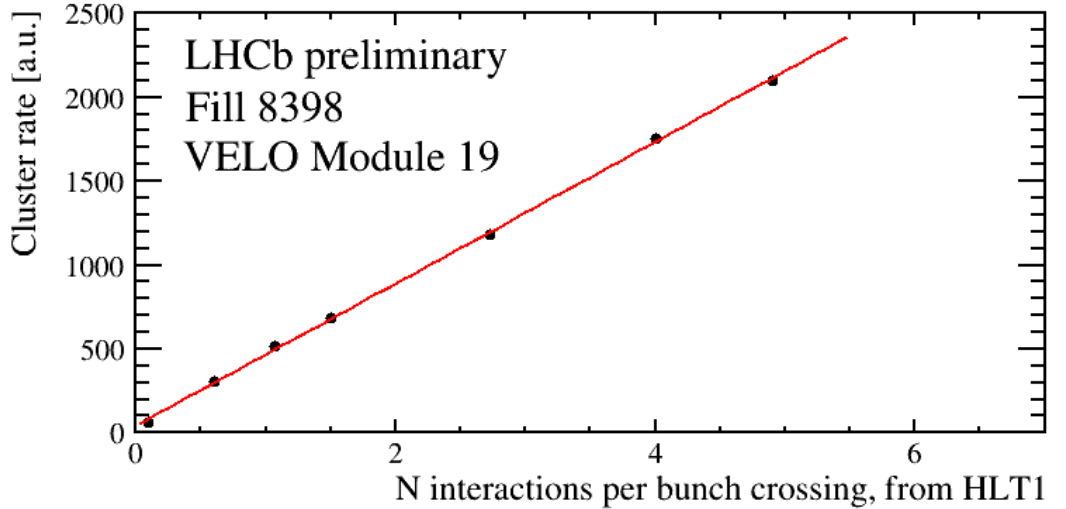
\includegraphics[width=0.8\textwidth]{figures/muscan.png}
    \caption{Linearity of cluster counters during mu-scan of November 2022}
    \label{fig:muscan}
\end{figure}


Absolute luminosity measurements are possible once the visible cross-section $\sigma_{vis}$ is known, allowing for an absolute luminosity value derived from the relative measurements $\mu_{vis}$. The visible cross-section $\sigma_{vis}$ are measured using the van der Meer scan, as described in Section \ref{sec:calibration_vdm}. In the next subsection, I will present the calibration that I performed using a vdM scan for each of the 208 counters.

Finally, I will present a robust procedure in order to combine the 208 different luminosity counters into a single luminosity measurement.

\subsection{Calibration of each counter with vdM scan}\label{sec:calibration_vdm}
Each of the 208 cluster counters is calibrated during the vdM scan independently. To explain the process, I will use the vdM scan conducted on September 7th, 2023, as an example.
It was a full 5 hours program with two symmetric scans and two 2-dimensional scans. Two additional symmetric and 2-dimensional scans alongside two Length Scale Calibrations (LSC) were performed with SMOG. The SMOG system\cite{CERN-LHCC-2019-005} injects a low flow rate of noble gas into the vacuum vessel of the VELO. This system is used to perform measurements in fixed-target mode and Beam-Gas-Imaging for measuring the beams position, shape and overlap integral\cite{Coombs:2767576}.. Figure \ref{fig:inner_vdm_sep} provides an overview of the vdM scan setup, illustrating the raw mean counts per event for the inner counters and the $x$ and $y$ positions of the two beams.

\begin{figure}
    \centering
    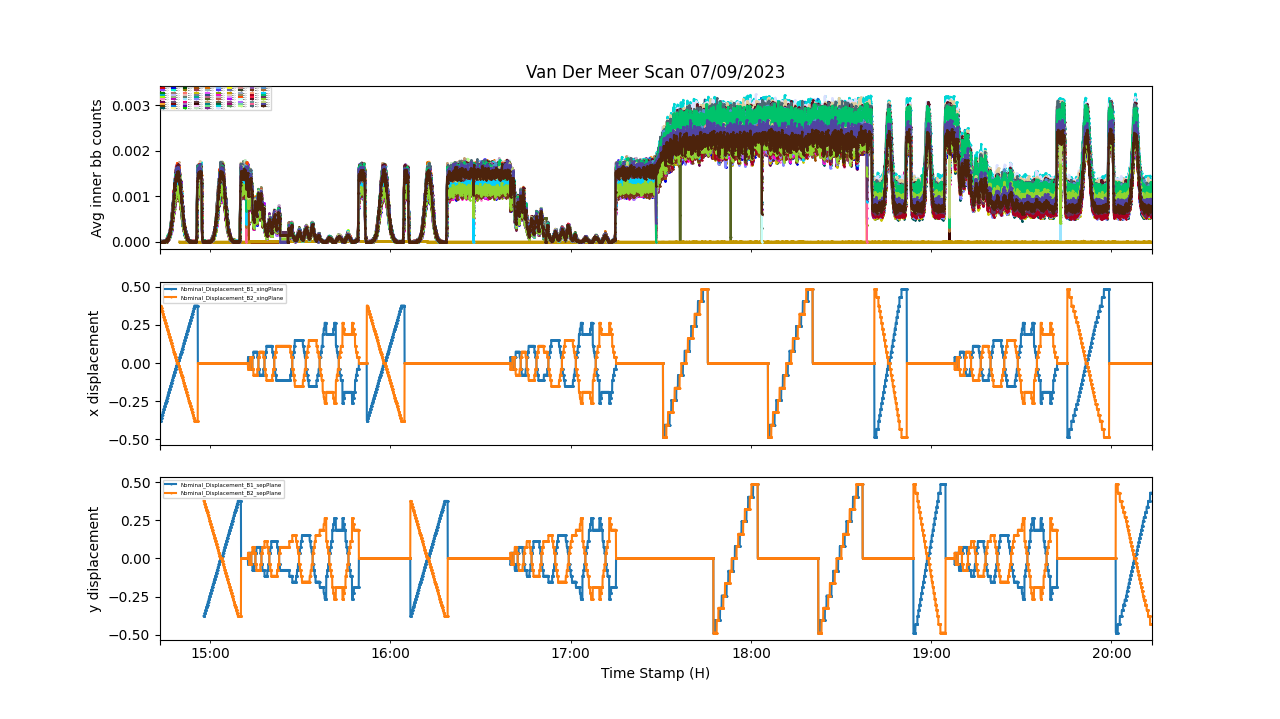
\includegraphics[width=\textwidth]{figures/inner_counts_bkg.png}
    \caption{Overview of the van der Meer scan of 7th September 2023. The first panel illustrates the raw mean counts per event of the 104 inner counters, while the second and third panels respectively depict the $x$ and $y$ positions of the two beams. Notice how an offset is introduced in the counters rate at $\approx$17:40 due to the SMOG injection.}
    \label{fig:inner_vdm_sep}
\end{figure}


During the initial phase of the scan, background noise was negligible, allowing the measurements to focus on the counts related to proton-proton ($pp$) interactions. Aan increase in the rate of the counters due to the injection of SMOG is clearly visible in Figure~\ref{fig:inner_vdm_sep}, around 17:30.  For the purpose of this thesis, SMOG introduces a background due to collisions of proton bunches with empty bunches, as seen in the ramp at 17:30 and increased occupancy of the counters.  As described in Section \ref{sec:velo_counters}, we implemented 4 different counters for each bunch crossing type, allowing the subtraction of the background in real time. However, in the calibration phase, this step is perfected offline. 

Another important step in the calibration involves normalising the counters to account for variations in the bunch population throughout the fill. This division allows for the estimation of the $\mu_{sp}$ defined in \eqref{mu_sp}. 

Figure \ref{fig:bkg_sub_calib} shows the corrected data with the background subtracted, highlighting in a purple box the vdM steps used in the calibration. These steps are, in chronological order, a symmetric X scan, a symmetric Y scan, and a 2D scan (or turtle scan). 

\begin{figure}
    \centering
    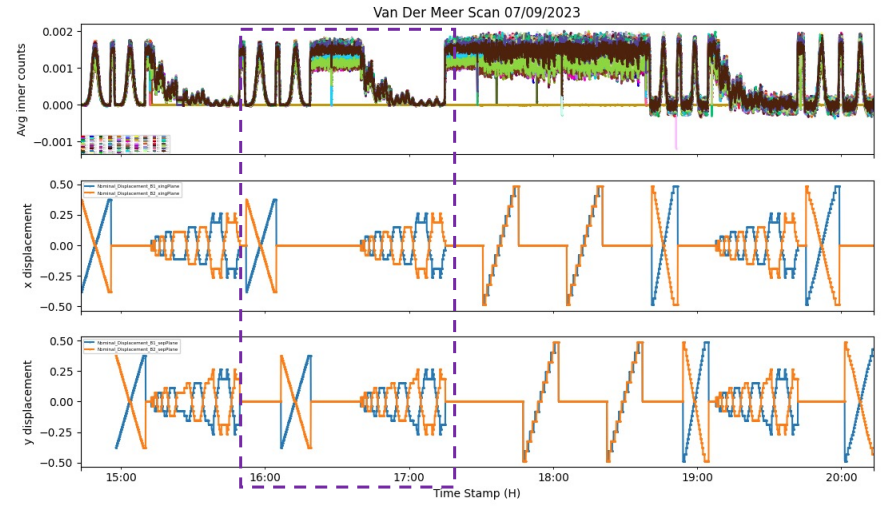
\includegraphics[width=\textwidth]{figures/calibration_period.png}
    \caption{Behaviour of the background-subtracted counters. No baseline is visible after 17:40, as it was in Figure \ref{fig:inner_vdm_sep}. The region used for the calibration is highlighted in the purple box. In this region a symmetric scan in X, a symmetric scan in Y, and a 2D scan were performed.}
    \label{fig:bkg_sub_calib}
\end{figure}

The calibration involves integrating the area under the counter data $\mu_{sp}$ as a function of $x$ and $y$ displacements, as described in \eqref{sigma_vdm}. We assume that the underlying density function for the distribution of the counts $\mu_{sp}(x,y)$ is a bivariate Gaussian, whose analytical form is given by Equation \eqref{2d-gaus}. 
\begin{equation}
    f(x,y|\mu_{x,y},\sigma_{x,y},\rho)=A\exp{\left(-{\frac {1}{2\left[1-\rho ^{2}\right]}}\left[\left({\frac {x-\mu _{X}}{\sigma _{X}}}\right)^{2}-2\rho \left({\frac {x-\mu _{X}}{\sigma _{X}}}\right)\left({\frac {y-\mu _{Y}}{\sigma _{Y}}}\right)+\left({\frac {y-\mu _{Y}}{\sigma _{Y}}}\right)^{2}\right]\right)}\label{2d-gaus}.
\end{equation}
Figure \ref{fig:fit_example} illustrates an example of such a 2D Gaussian fit, along with the corresponding residuals. The $\chi^2$ reported in the figure assesses the validity of the 2D-Gaussian modelling, being this statistic of goodness-of-fit within $1$ standard deviation from its expected value (i.e. the number of degree of freedom DF).


\begin{figure}
    \centering
    \begin{subfigure}{0.48\textwidth}
    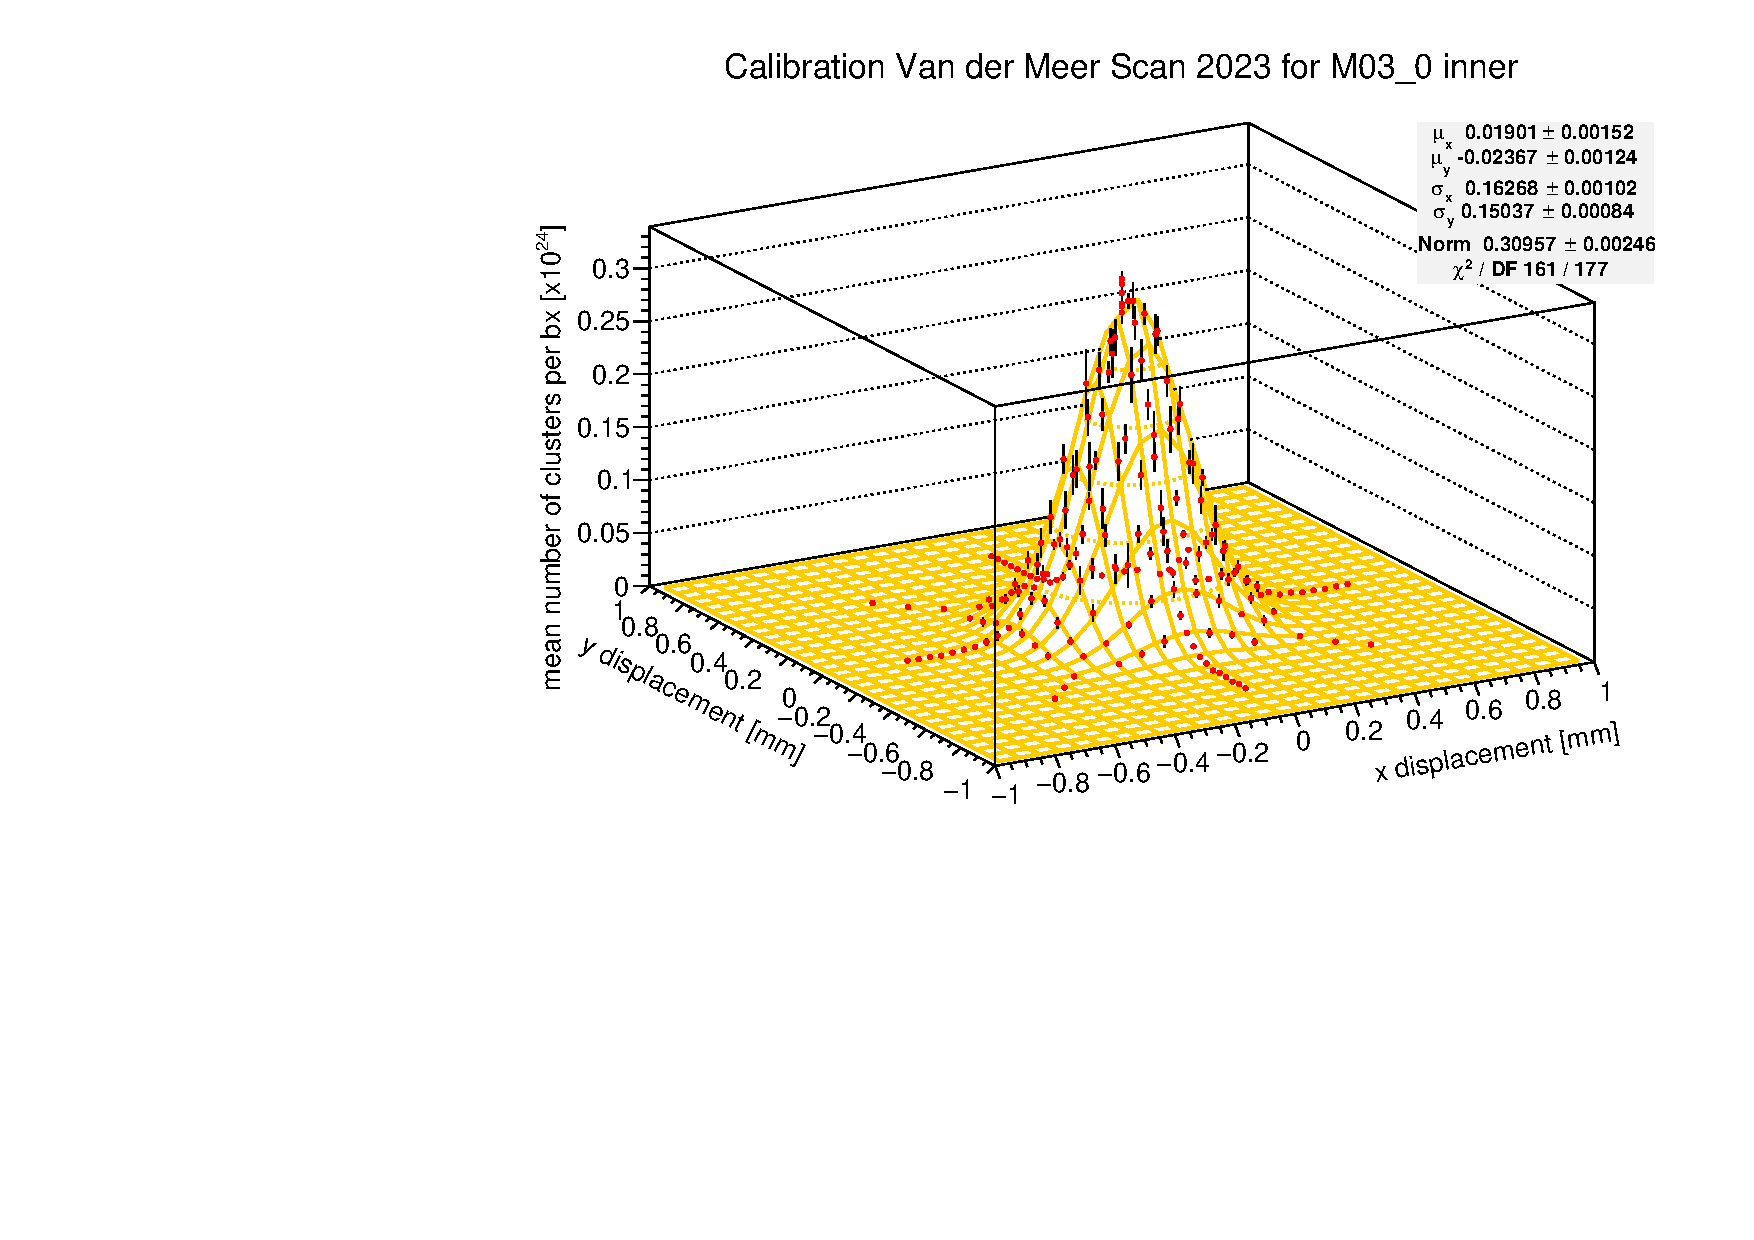
\includegraphics[width=\linewidth]{figures/M03_0.pdf}
    \caption{2D Gaussian fit to the counter M$03\_0$ inner}\label{fig:fit_M03}
    \end{subfigure}
    \begin{subfigure}{0.48\textwidth}
    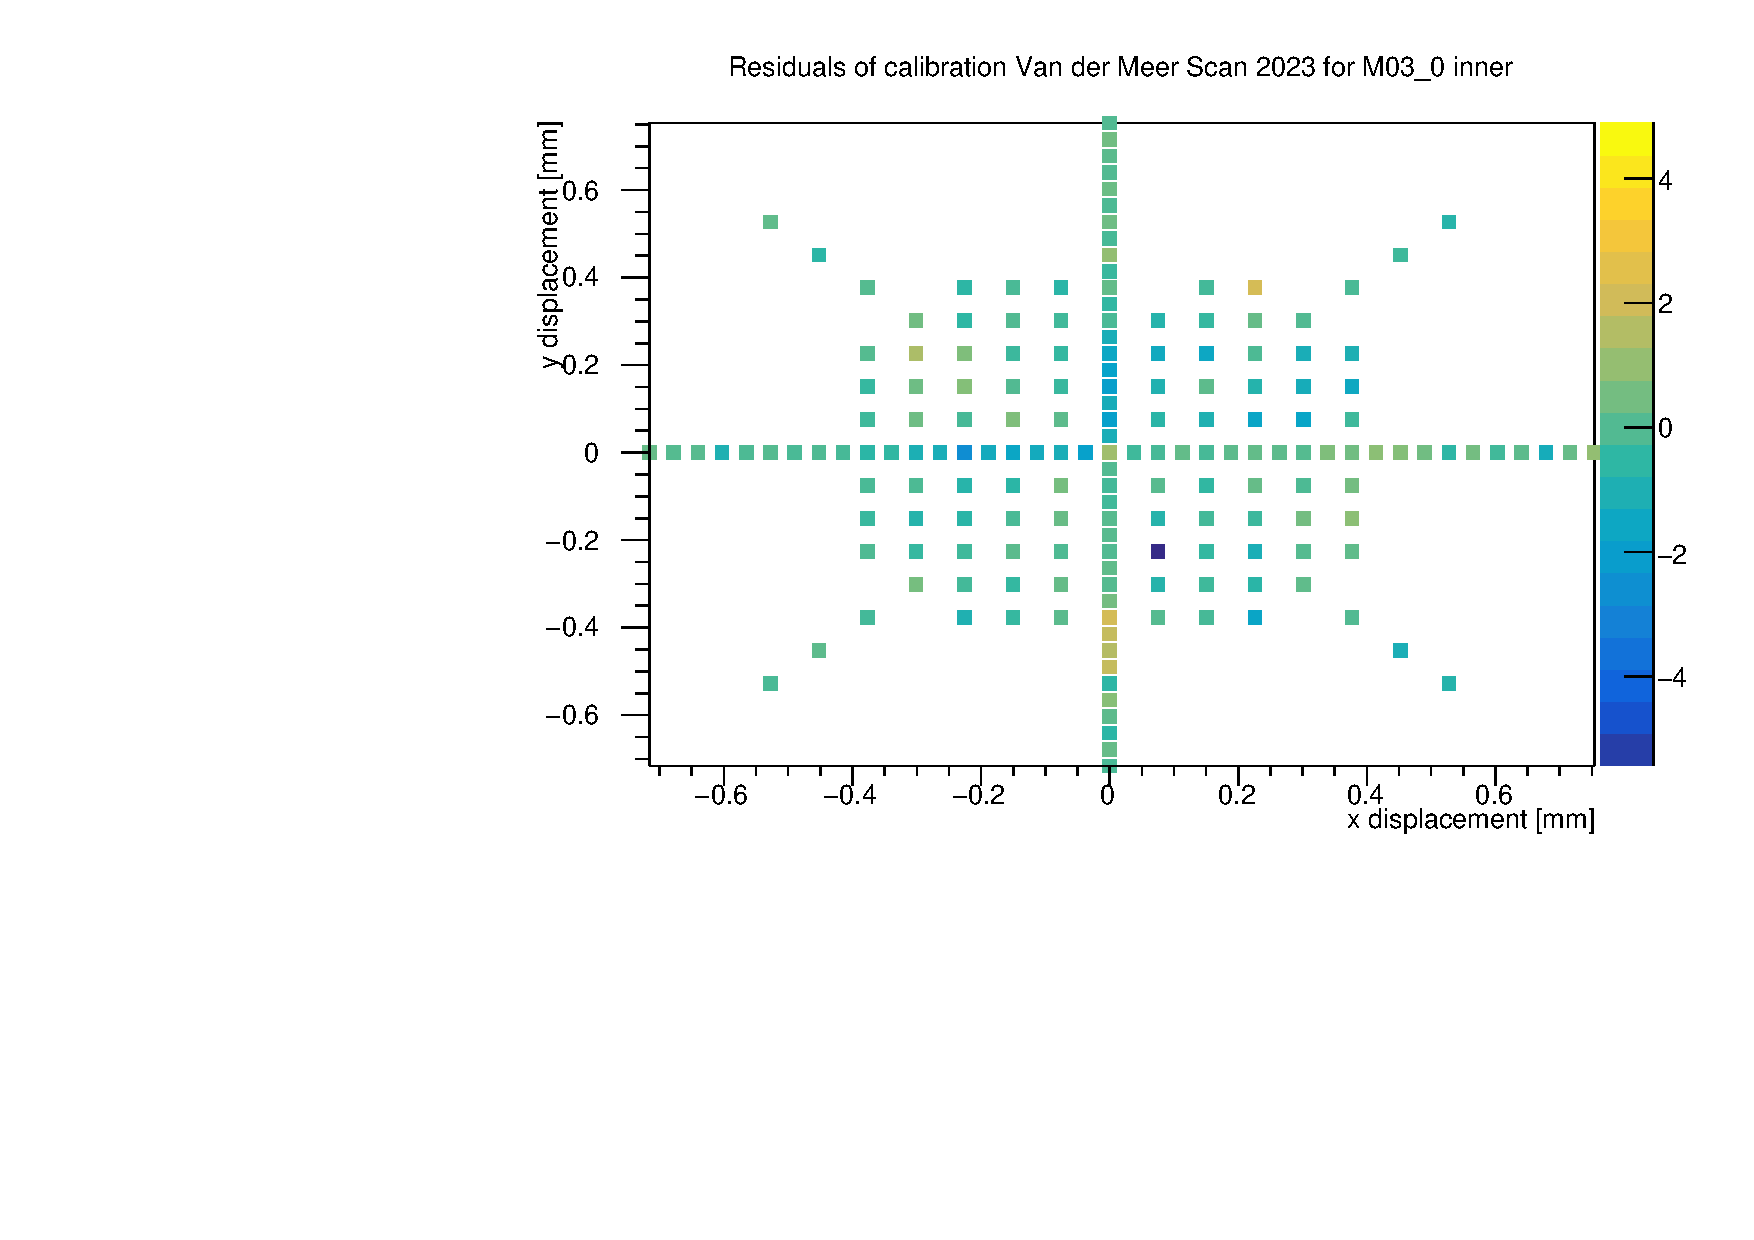
\includegraphics[width=\linewidth]{figures/M03_0_res.pdf}
    \caption{Residuals of the fit}\label{fig:M03_res}
    \end{subfigure}
    \caption{Example of a 2D Gaussian fit to perform the calibration on one the inner counter of the third module during the van der Meer scan. The same procedure is repeated for each counter. On the left, the measurements of the mean counts at a specific displacement in $x$ and $y$ is displayed in red. At each point a black error bar is associated accounting for the standard deviation of the different measurements in the same position as well as the Poisson uncertainty. The yellow surface is the fitte 2D Gaussian of equation~\eqref{2d-gaus}. On the right, a two dimensional representation of the residuals of the fitted function with respect to measurements is displayed. The residuals are color-coded to present the missing 3rd dimensional axis.}
    \label{fig:fit_example}
\end{figure}

The integral of the function in equation~\eqref{2d-gaus} is computed to obtain the normalisation factor: 
\begin{equation}
    N = 2\pi A \sigma_{X}\sigma_{Y}\sqrt {1-\rho ^{2}}=\sigma_{vis},\label{2d-gaus-norm}
\end{equation}
This normalisation factor represents the visible cross section, $\sigma_{vis}$, which is the quantity that we need to to calculate for perform the calibration.

 The results of each $\sigma_{vis}$ are reported as a function of the $z$ position of the module in Figure \ref{fig:coefficient_pos}, demonstrating how the calibration varies depending on the position along the detector $z$-axis.

\begin{figure}
    \centering
    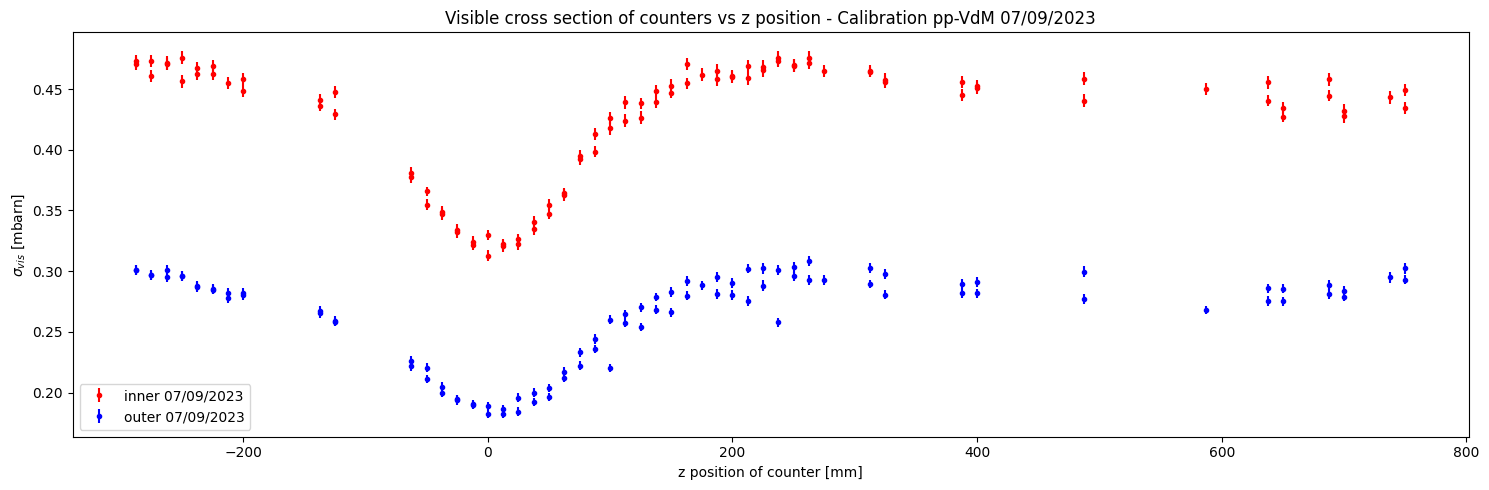
\includegraphics[width=\textwidth]{figures/coefficient_pos.png}
    \caption{Measured $\sigma_{vis}$ for each counter, as a function of the counter position along the $z$-axis of the detector. The shape around $z=0$ is expected due to the VELO acceptance, and it was previously observed in simulation.}
    \label{fig:coefficient_pos}
\end{figure}

Once the visible cross section $\sigma_{vis}$ is calculated for each counter, each of them can provide a luminosity estimation based on the definition in \eqref{rel_lumi}.

\subsection{Combining the counters for into a luminosity measurement}
We face now the issue of how to combine the counters for a single, more precise, luminosity measurement. In fact, the calibration with the vdM scan allowed to calculate a calibration factor for every counter, yielding 208 different luminosity measurements. 
First off, the question is how all the different measurement at the same timestamp are distributed. 
This is reported in Figure \ref{fig:lumi_hist_ts} at two different timestamps spaced by 15 minutes for data collected during the vdM scan of September 7th 2023. The distribution is not a perfect Gaussian, but mean and standard deviation are robust metrics to describe the peak and the width of the curve. 


\begin{figure}
    \centering
    \begin{subfigure}{0.48\textwidth}
    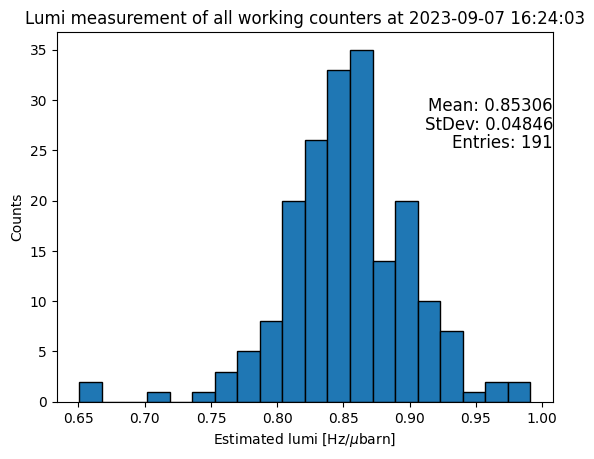
\includegraphics[width=\linewidth]{figures/lumi_hist_1624.png}
    \caption{Timestamp 16:24}\label{fig:lumi1624}
    \end{subfigure}
    \begin{subfigure}{0.48\textwidth}
    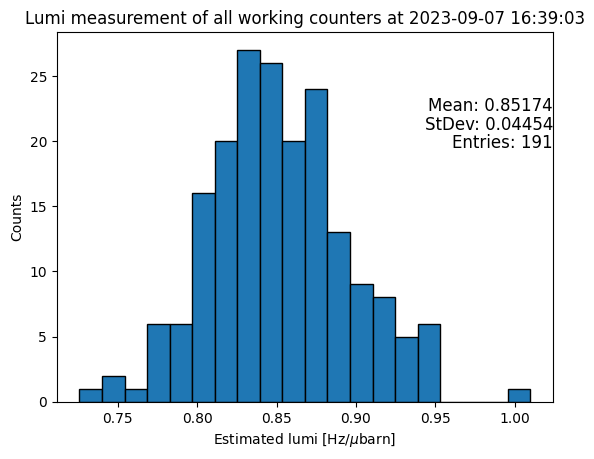
\includegraphics[width=\linewidth]{figures/lumi_hist_1639.png}
    \caption{Timestamp 16:39}\label{fig:lumi1639}
    \end{subfigure}
    \caption{Distribution of the luminosity estimates of all the working counters during the vdM scan fill of 7th September 2023. Two different timestamps are reported at a distance of 15 minutes one to the other. The entries are 191 instead of 208, due to various counters not working during vdM.}
    \label{fig:lumi_hist_ts}
\end{figure}

In fact, we see in the trace plots of Figure \ref{fig:std_dev_rel_std} (left) that the standard deviation of the luminosity estimations is proportional to the luminosity estimation. This encourages us to study the relative standard deviation defined as the standard deviation $\sigma$  divided by the mean $\mu$:
\begin{equation}
    \sigma_{rel} = \frac{\sigma}{\mu} \label{rel_std}.
\end{equation}


\begin{figure}
    \centering
    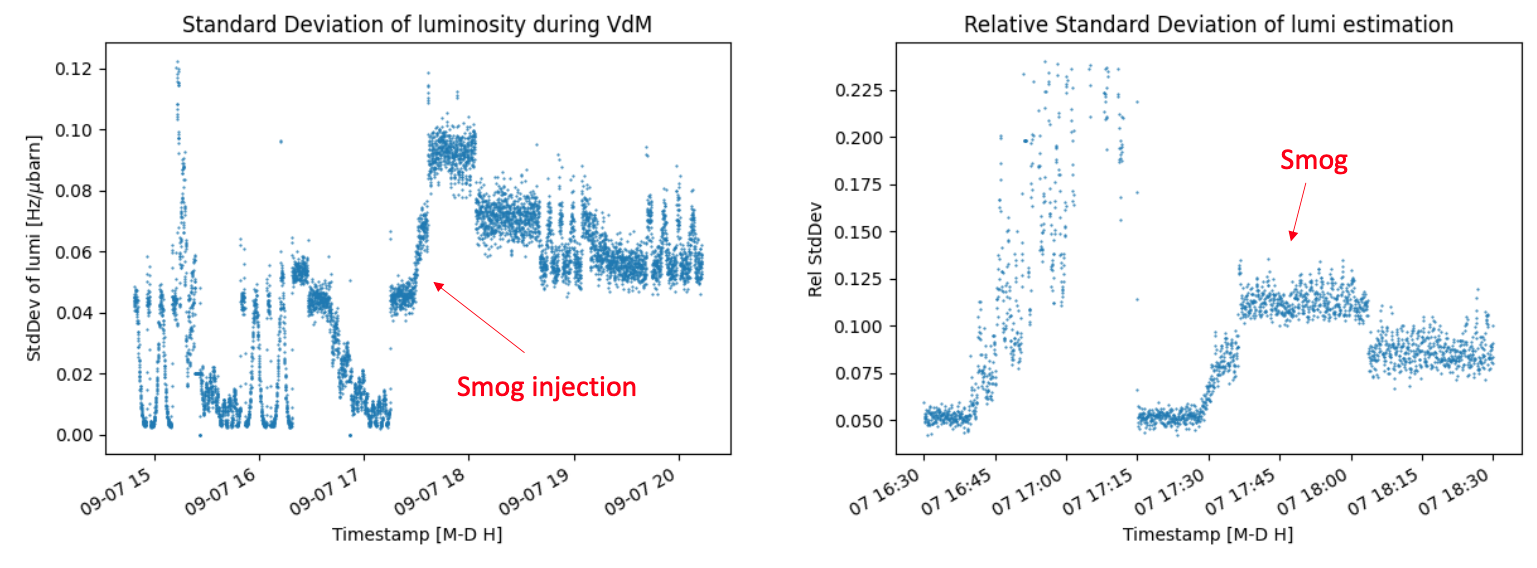
\includegraphics[width=\textwidth]{figures/std_dev_and_rel_std.png}
    \caption{Standard deviation (left) and relative standard deviation (right) of the luminosity estimators during the vdM fill. Notice how this increase after the injection of SMOG at $\approx$17:40}
    \label{fig:std_dev_rel_std}
\end{figure}


The relative standard deviation $\sigma_{rel}$ is plotted as a function of time in Figure \ref{fig:std_dev_rel_std} (right). One notices that the value is stable at 5\% except for the period when the gas from SMOG is injected in the vacuum chamber (around 17:30) and for the time when the mean value $\mu$ of the luminosity is approximately zero (between 16:45 and 17:15).  

This study assures us that the calibration is stable in the short term, and that all the counters provide a reasonable luminosity measurement. However, when combining a large set of measurements, it is critical to choose an appropriate estimator to ensure that the final result is robust. With a dataset containing 208 individual measurements, the presence of outliers or deviations from the assumed probability distribution cannot be excluded. Consequently, choosing a robust estimator becomes essential to mitigate the impact of such anomalies.

Robustness in statistics refers to the ability of an estimator to resist the influence of outliers and remain relatively stable under deviations from distribution assumptions. A robust estimator does not significantly change due to a small number of atypical values or when the distribution deviates from its presumed normality.

In this context, I tested the performance of three different estimators to determine the best approach for combining my measurements: the mean, the median, and the trimmed mean. Each estimator has its strengths and weaknesses in terms of robustness.

\begin{itemize}
\item Mean: the mean is a common estimator, but it is highly sensitive to outliers. Even a single extreme value can significantly skew the result, making it less suitable for datasets with potential anomalies.
\item Median: the median, which represents the middle value in a dataset, is inherently robust because it is not influenced by outliers. It is often used when the data distribution is skewed or when outliers are present.
\item Trimmed Mean: the trimmed mean is a compromise between the mean and the median. It involves removing a specified percentage of the largest and smallest values from the dataset before calculating the mean. This approach retains some of the data central tendency while reducing the effect of extreme values.
\end{itemize}


An overview of the behaviour of these three estimators during the vdM is plotted in Figure \ref{fig:lumi_estimator_location_param}. By eye, the behaviour of the three estimators in Figure \ref{fig:comparison_whole} is very similar to one another. However, in a zoomed region such as the one in Figure \ref{fig:comparison_zoom} one can notice how sudden drops in luminosity are differently registered by the tested estimators. Otherwise, the behaviour of these three estimators does not really change.
 

\begin{figure}
    \centering
    \begin{subfigure}{0.48\textwidth}
    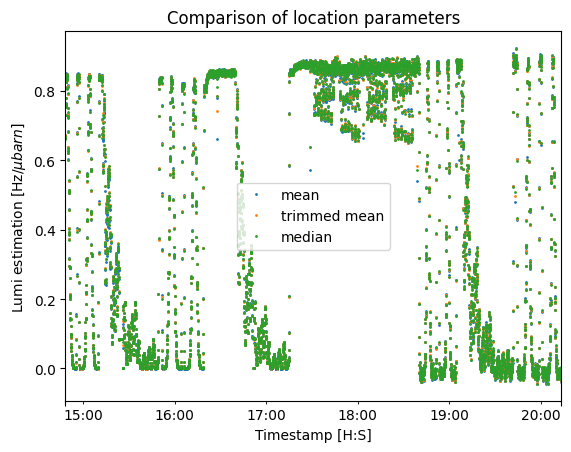
\includegraphics[width=\linewidth]{figures/comparison_location_whole.png}
    \caption{Whole fill}\label{fig:comparison_whole}
    \end{subfigure}
    \begin{subfigure}{0.48\textwidth}
    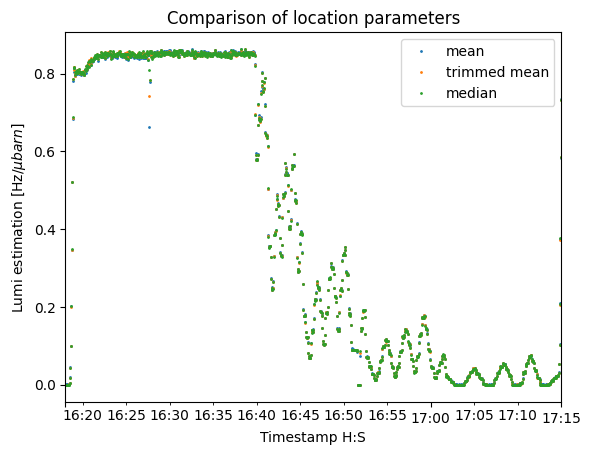
\includegraphics[width=\linewidth]{figures/comparison_location.png}
    \caption{Zoom on constant region and 2D scan}\label{fig:comparison_zoom}
    \end{subfigure}
    \caption{Comparison of three possible global luminosity estimators over the vdM data. In green: median, in blue: mean, in orange: trimmed mean (15\%)}
    \label{fig:lumi_estimator_location_param}
\end{figure}

In order to test the performances of these estimators, I selected a region during the vdM scan when the luminosity should be constant in time. Then, I fitted an horizontal line (Figure \ref{fig:costant_fit_location}) and computed the residuals of each estimator with respect to the fitted constant. By observing the standard deviation of the distribution of the residuals shown in Figure \ref{fig:res_location}, we can evaluate the precision in time of each estimator. All three of them performed similarly, yielding a luminosity resolution of 0.5\% every 3 seconds of data taking.

I found that the median and the trimmed mean were more robust estimators compared to the mean. Given the potential for outliers and the uncertainty in the underlying probability distribution, I selected the trimmed mean at 15\% as the most appropriate estimator for my final analysis. This choice was also based on the fact that the trimmed mean has a slightly better resolution, as shown in the residuals displayed in Figure~\ref{fig:res_location}. The trimmed mean also provides a balance between the stability of the median and the information content of the mean, ensuring a reliable estimate while minimising the influence of outliers.

\begin{figure}
    \centering
    \begin{subfigure}{0.48\textwidth}
    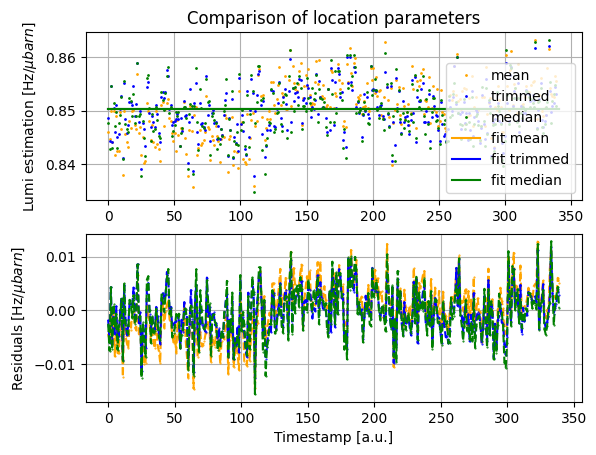
\includegraphics[width=\linewidth]{figures/fit_wo_outliers.png}
    \caption{Constant fit}\label{fig:costant_fit_location}
    \end{subfigure}
    \begin{subfigure}{0.48\textwidth}
    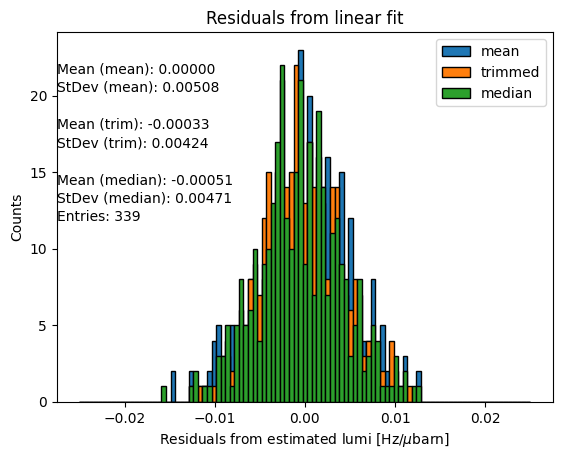
\includegraphics[width=\linewidth]{figures/resiudals_without_outliers.png}
    \caption{Residuals}\label{fig:res_location}
    \end{subfigure}
    \caption{Comparison of three possible location parameter over a stable region of luminosity}
    \label{fig:lumi_fit_location_param}
\end{figure}

The value of the chosen estimator (the trimmed mean) is depicted as a function of time during the vdM scan in the second panel of Figure \ref{fig:lumi_result_all}. The drops seen during the LSC scans are due to the fact that the beams do not always collide head to head. In fact, one beam is shifted asynchronously with respect to the other, leading to a smaller overlap between the beams and therefore lower luminosity. 

Figure \ref{fig:lumi_result_all} provides a good summary of my analysis of this vdM scan. In the first panel the average background-subtracted counts of each counter is reported, while on the third and fourth panel the movements of the two beams in the $x$ and $y$ direction are depicted, respectively.

\begin{figure}
    \centering
    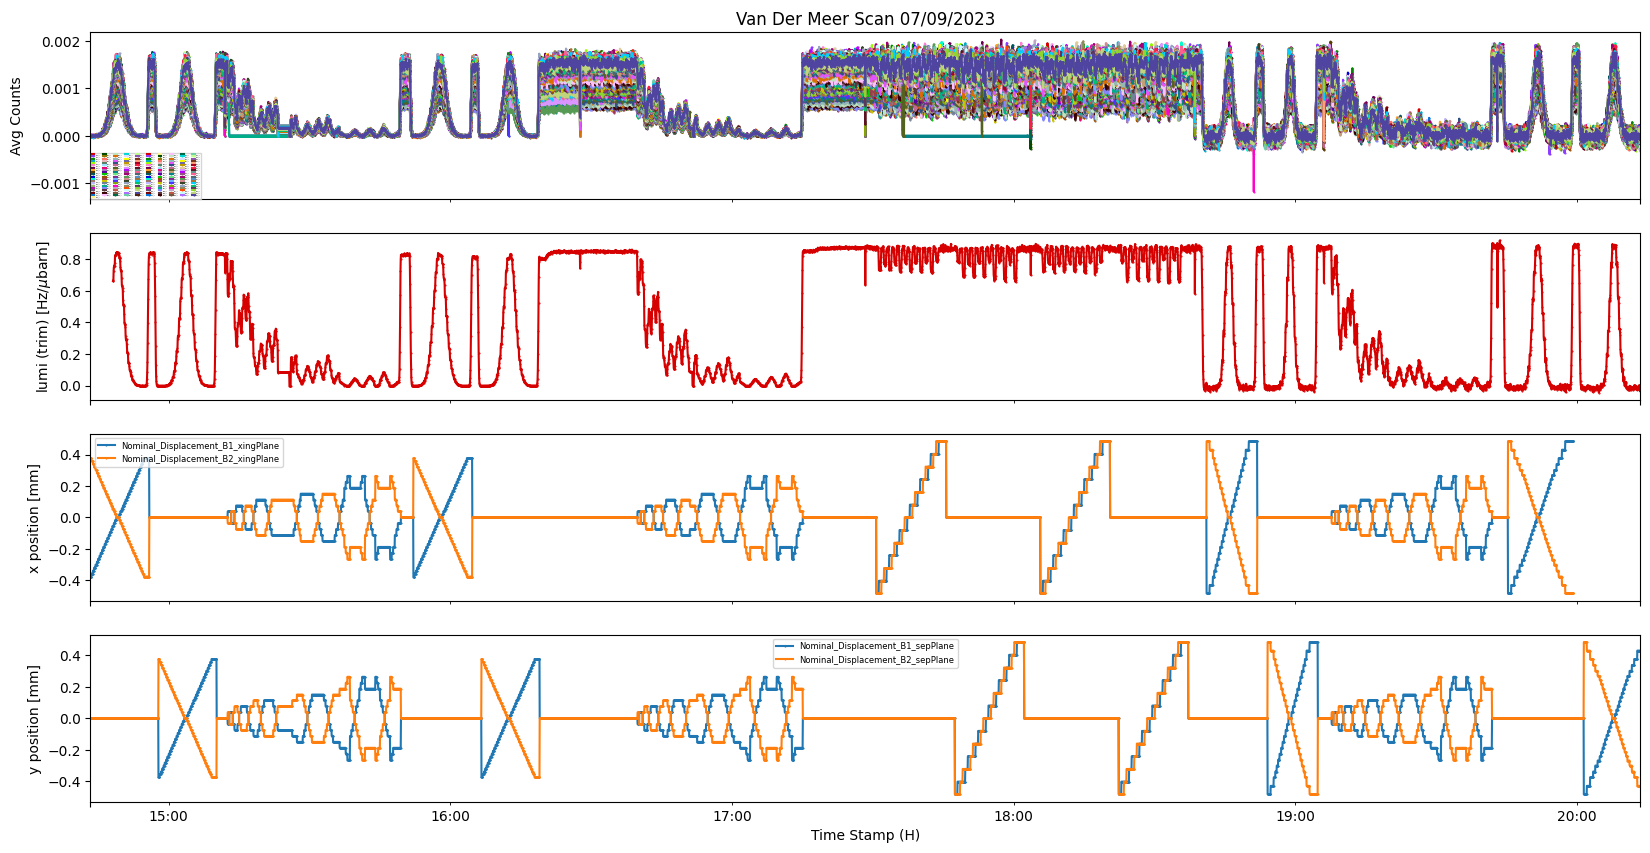
\includegraphics[width=\textwidth]{figures/lumi_plot.png}
    \caption{Value of of the luminosity estimator [second panel] during the vdM scan conducted on 07/09/23.
The first panel illustrates the background-subtracted mean counts per event of the 208 counters, while the third and fourth
panels respectively depict the $x$ and $y$ positions of the two beams.}
    \label{fig:lumi_result_all}
\end{figure}

Once the luminosity estimation is available, we can compute the instantaneous $\mu$ similarly to equation $\eqref{mu_def}$ by using the cross section $\sigma_{LHCb}~=~\SI{62.2}{\milli\barn}$ for $pp$ inelastic scattering at $\sqrt{s}~=~\SI{14}{\tera\eV}$~\cite{Aaij:2310870}:
\begin{equation}
    \mu = \frac{\mathcal{L}\sigma_{LHCb}}{f N_b}\label{inst_mu}
\end{equation}




To evaluate the medium term stability of the calibration from September 7th, 2023, we estimated the luminosity for Fill 9168, which took place on September 17th, 2023. This estimation used the visible cross-section $\sigma_{vis}$ derived from the vdM scan described in this chapter. Figure \ref{fig:fill9168} provides an overview of the results from this study.
\begin{figure}
    \centering
    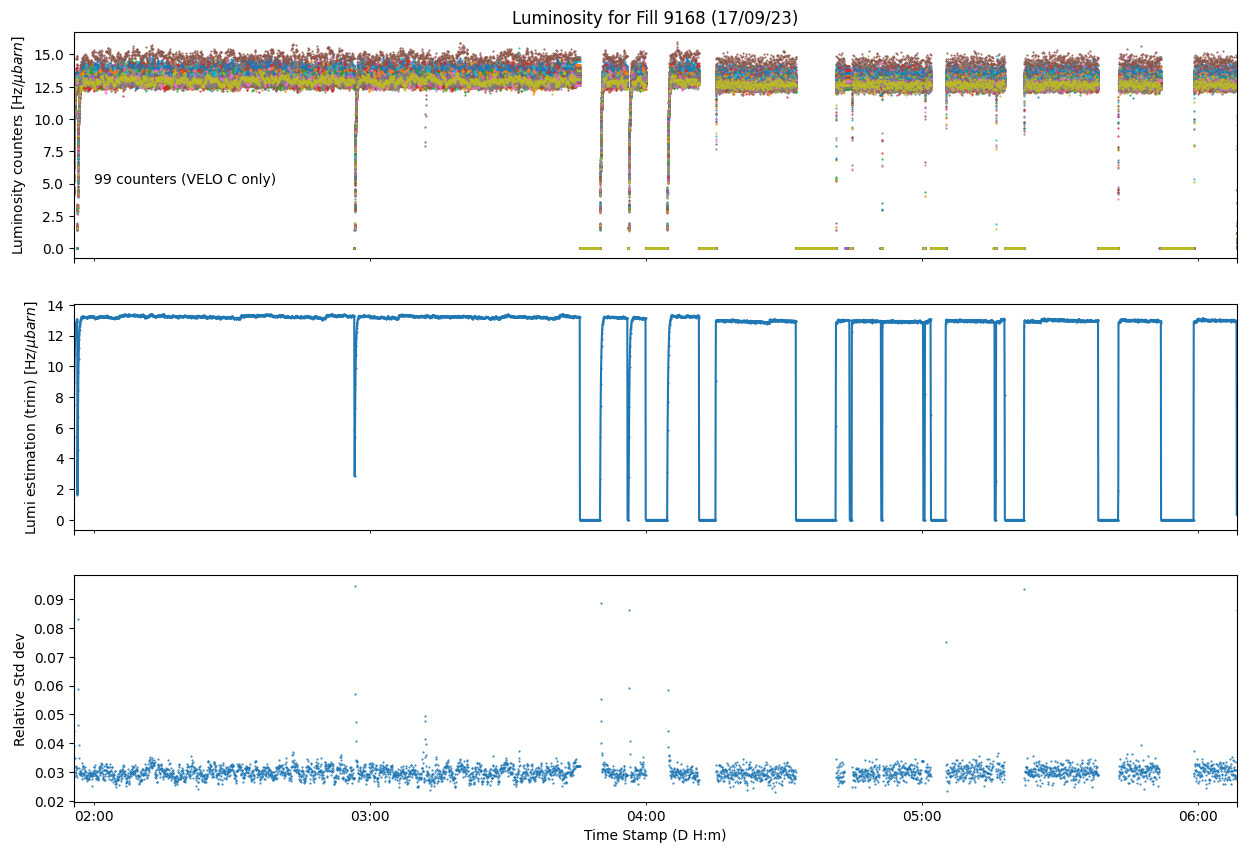
\includegraphics[width=\textwidth]{figures/fill9168.png}
    \caption{Luminosity during Fill 9168.}
    \label{fig:fill9168}
\end{figure}
In the first panel of Figure \ref{fig:fill9168}, the luminosity readings from each individual counter are displayed. Unfortunately, during this fill, only the C side of the VELO was operational, reducing our available data and resulting in a significant drop in statistics. The second panel shows the combined luminosity estimate, calculated as the trimmed mean of the functioning counters. The sudden drops are due to a restart of the LHCb run.  The third panel displays the relative standard deviation of the luminosity measurements for each counter. As seen in the figure, the relative standard deviation stabilises at around 3\%. This value is slightly better than the 5\% observed during the vdM scan. The difference between these two value is due to the difference in the number of working counters in the two fills. In fact, in the vdM fill 191 counters were working, while in Fill 9168 we had only 99 working counters. We therefore expect that the standard deviation should reduce by a factor $\sqrt{99/191}=0.7$, i.e. which is the factor binding 5\% with 3\%.

Despite the reduced data due to limited VELO operation, the relative stability of the combined luminosity estimate indicates that the calibration from the earlier vdM scan remains reliable in the medium term. The consistency of the relative standard deviation suggests that the estimation method is robust, even with a reduced sample size, providing confidence in the calibration effectiveness across different datasets and time periods.
Furthermore, we can evaluate a global uncertainty on the estimator. Since we observe a relative standard deviation of 3\%, stable in time, we can define the uncertainty by dividing this value by the squared root of the number of counters, in this case given by the 99 operational counters. Therefore, the relative uncertainty quoted of the trimmed mean estimator corresponds to approximately 0.3\%. For comparison, in Run~2 the precision obtained offline after a careful analysis and cross-calibration of \textit{all} the available counters in LHCb was 0.2\%~\cite{lumi2}.